\section{Runtime Algorithms: Conditional Memory, Embeddings, Stability, and Inference Routing}
\label{sec:annex-runtime}

This annex collects the runtime algorithms that support the configuration-driven pipeline: conditional memory (Engram), factorized embeddings and embedding convolution, training-step stability controls, the held-out evaluation split, and the SBERT inference mode router. Bibliography keys cited here resolve against \texttt{docs/bibliography/}.

\subsection{Engram Conditional Memory}

\begin{figure}[H]
\centering
\fitfigure{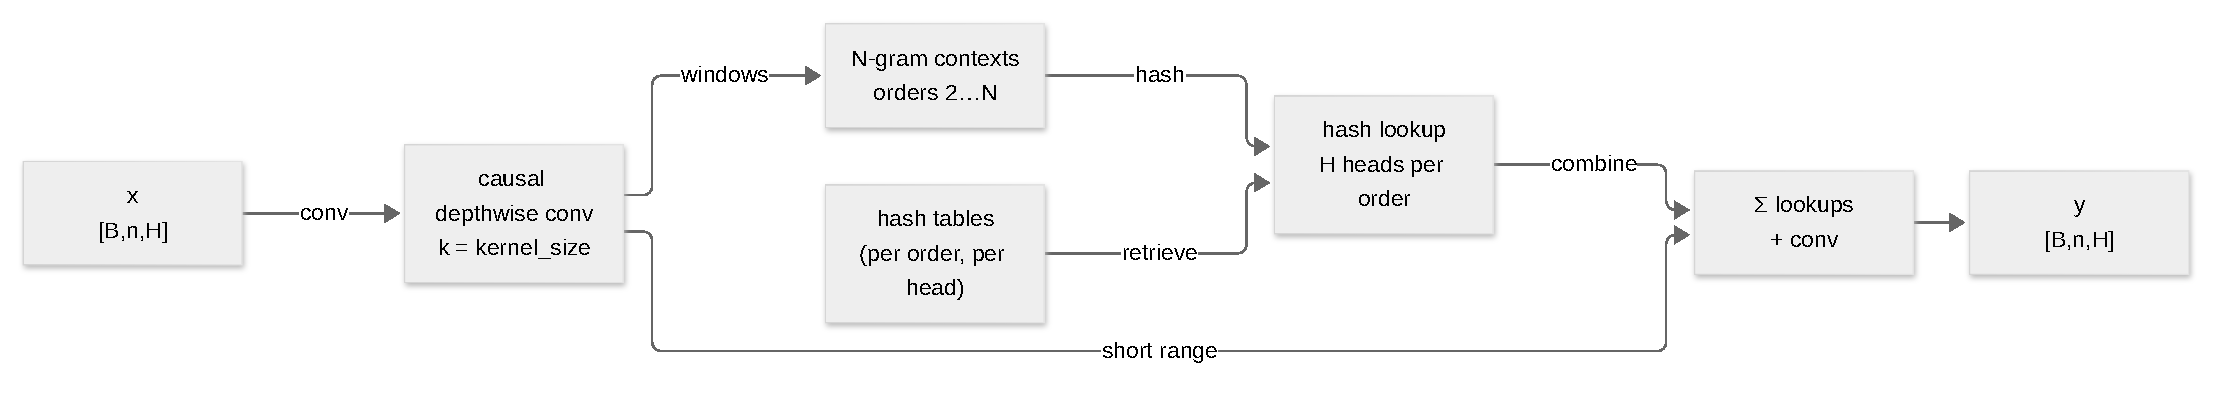
\includegraphics{figures/mixers/engram.pdf}}
\caption{Dataflow of Engram conditional memory: a causal depthwise convolution supplies short-range context, N-gram hash lookups retrieve per-order embeddings, and the lookups are summed with the convolution output.}
\label{fig:mixer-engram}
\end{figure}

Engram (\texttt{engram}) implements conditional memory via scalable N-gram lookup \citep{cheng2026conditionalmemoryscalablelookup}. It builds hash-based lookup tables for N-gram contexts from size 2 up to \texttt{engram\_max\_ngram\_size}, with independent hash heads per N-gram order. A causal depthwise convolution (\texttt{engram\_kernel\_size}) provides short-range context before the N-gram lookup.

\begin{algorithmic}[1]
\State \textbf{Input:} token stream $x_{1:n}$, N-gram orders $\{2, \ldots, N\}$, hash heads per order $H$
\State $h_{\text{conv}} \gets \text{DepthwiseConv1d}(x_{1:n}, k=\texttt{engram\_kernel\_size})$ \Comment{short-range context}
\For{each N-gram order $k \in \{2, \ldots, N\}$}
    \State $\text{ctx}_t^{(k)} \gets x_{t-k+1:t}$ \Comment{N-gram context window}
    \State $\text{lookup}^{(k)}_t \gets \text{HashTable}^{(k)}[\text{hash}(\text{ctx}_t^{(k)})]$ \Comment{per-head retrieval, $H$ heads per order}
\EndFor
\State $y_t \gets \sum_{k} \text{lookup}^{(k)}_t + h_{\text{conv},t}$ \Comment{combine conditional memories}
\State \textbf{Output:} $y_{1:n}$
\end{algorithmic}

\subsubsection{Configuration}
\begin{itemize}[leftmargin=*]
    \item \texttt{engram\_max\_ngram\_size}: int $\ge 2$ --- highest N-gram order (default 3).
    \item \texttt{engram\_n\_heads\_per\_ngram}: int $\ge 1$ --- hash heads per N-gram order (default 4).
    \item \texttt{engram\_embed\_dim\_per\_head}: int $\ge 1$ --- embedding dim per hash head (default 32).
    \item \texttt{engram\_kernel\_size}: int $\ge 1$ --- causal depthwise conv kernel width (default 4).
    \item \texttt{engram\_seed}: int --- hash seed for reproducibility (default 42).
\end{itemize}
Total Engram hidden size = $(\texttt{max\_ngram\_size} - 1) \times \texttt{n\_heads\_per\_ngram} \times \texttt{embed\_dim\_per\_head}$.

\subsection{Factorized Embeddings and Embedding Convolution}

\subsubsection{Factorized Embeddings}
When \texttt{use\_factorized\_embedding=true}, the embedding matrix is factorized into two smaller matrices, reducing parameters from $O(V \times H)$ to $O(V \times R + R \times H)$ where $R = \texttt{factorized\_embedding\_dim}$.
\begin{itemize}[leftmargin=*]
    \item \texttt{use\_factorized\_embedding}: bool --- enable factorization.
    \item \texttt{factorized\_embedding\_dim}: int $\ge 1$ --- intermediate dimension (typical: 64--256).
\end{itemize}

\subsubsection{Embedding Convolution}
When \texttt{use\_embedding\_conv=true}, a depthwise Conv1d is applied over the embedding stream before the first transformer block, with kernel size \texttt{embedding\_conv\_kernel}. This provides a lightweight local-context filter on token embeddings.

\subsection{Training-Step Stability Controls}

The schema-driven training step applies gradient accumulation, global-norm clipping, post-clip explosion guards, and bounded NaN/Inf retries. The accumulated gradient is:
\[
g_{\text{acc}}=\frac{1}{K}\sum_{i=1}^{K} g_i,\quad K=\texttt{gradient\_accumulation\_steps}
\]
\[
g_{\text{clip}} = g_{\text{acc}}\cdot
\min\left(1,\frac{\tau}{\|g_{\text{acc}}\|_2+\epsilon}\right),\quad
\tau=\texttt{grad\_clip\_max\_norm}
\]
then overflow guards use \texttt{inf\_post\_clip\_threshold} and retry logic bounded by \texttt{max\_nan\_retries}.

\begin{algorithm}[t]
\caption{Schema-Driven Training Step with Stability Controls}
\begin{algorithmic}[1]
\Require Batch stream, config $C$
\State Initialize retry counter $r\gets 0$
\For{each optimizer step}
    \State Accumulate gradients for $K=C.\texttt{gradient\_accumulation\_steps}$ micro-batches
    \State Apply global norm clipping with $\tau=C.\texttt{grad\_clip\_max\_norm}$
    \If{post-clip gradient exceeds $C.\texttt{inf\_post\_clip\_threshold}$ or NaN/Inf detected}
        \If{$r < C.\texttt{max\_nan\_retries}$}
            \State restore safe state / skip step; $r \gets r+1$
            \State \textbf{continue}
        \Else
            \State stop training with failure state
        \EndIf
    \EndIf
    \State run optimizer step selected by \texttt{optimizer\_class}
    \State update scheduler (\texttt{cosine}, \texttt{constant}, or \texttt{linear\_warmup\_then\_constant})
    \If{step mod \texttt{checkpoint\_every\_n\_steps}$=0$}
        \State save rolling checkpoint and prune to \texttt{max\_rolling\_checkpoints}
    \EndIf
    \State update best checkpoints up to \texttt{num\_best\_checkpoints}
    \State emit CSV + telemetry following \texttt{gradient\_log\_interval} and \texttt{telemetry\_log\_interval}
\EndFor
\end{algorithmic}
\end{algorithm}

\subsection{Held-Out Test Split and End-of-Training Evaluation}

\texttt{training.test\_percentage} reserves a deterministic fraction of the task dataset before the first optimizer step. With $n$ dataset examples, held-out percentage $\rho=\texttt{test\_percentage}/100$, and a permutation $\pi$ drawn once from the run seed \texttt{training.seed}, the partition is
\[
n_{\text{test}}=\operatorname{clip}\!\left(\operatorname{round}(\rho n),\,1,\,n-1\right),\qquad
\mathcal{D}_{\text{train}}=\{x_{\pi(i)}\}_{i=n_{\text{test}}+1}^{n},\qquad
\mathcal{D}_{\text{test}}=\{x_{\pi(i)}\}_{i=1}^{n_{\text{test}}} ,
\]
so the same configuration always reserves the same examples regardless of DataLoader shuffling. After the last epoch the final weights are evaluated once with the task objective under \texttt{no\_grad}, and the sample-weighted loss and accuracy
\[
\hat{L}=\frac{1}{n_{\text{test}}}\sum_{x\in\mathcal{D}_{\text{test}}}\ell(f_\theta;x),\qquad
\widehat{\text{acc}}=\frac{1}{n_{\text{test}}}\sum_{x\in\mathcal{D}_{\text{test}}}a(f_\theta;x)
\]
are written to \texttt{test\_metrics.json} next to the CSV log. The split covers masked and causal language modeling, text classification, the three vision tasks, ASR (where the accuracy slot carries the character error rate, labelled \texttt{metric: cer}), and audio classification. SBERT keeps its own validation partition through \texttt{training.sbert.max\_eval\_samples} and is unaffected. Setting the field to zero disables the split and restores the historical all-data behavior.

\subsection{SBERT Inference Mode Router}

The SBERT inference dispatcher selects among similarity scoring, corpus search, clustering, and persistent encoding modes over a single shared encoder \citep{reimers_sentence-bert_2019}. The cosine similarity and regression loss are:
\[
\text{cos}(e_1,e_2)=\frac{e_1^\top e_2}{\|e_1\|\|e_2\|},\qquad
\mathcal{L}_{\text{cos}}=\left(\text{cos}(e_1,e_2)-y\right)^2
\]
with $y\in[-1,1]$ in this pipeline.

\begin{algorithm}[t]
\caption{SBERT Inference Mode Router}
\begin{algorithmic}[1]
\Require mode $m$, model $E$, inputs $X$
\If{$m=\texttt{similarity}$}
    \State return $\cos(E(x_1),E(x_2))$
\ElsIf{$m=\texttt{search}$}
    \State return top-$k$ by dot-product/cosine against corpus embeddings
\ElsIf{$m=\texttt{cluster}$}
    \State return clustering labels over $E(X)$
\Else
    \State return serialized embeddings $E(X)$
\EndIf
\end{algorithmic}
\end{algorithm}